\documentclass[11pt]{article}
\usepackage[margin=3cm]{geometry}
\usepackage[swedish]{babel}
\usepackage[utf8]{inputenc}
\usepackage[T1]{fontenc}
\usepackage{fancyhdr}
\usepackage{ragged2e}
\usepackage{titling}
\usepackage{graphicx}
\usepackage{pbox}
\usepackage{tabularx}
\usepackage{longtable}
\usepackage{tabu}
\usepackage{url}

\graphicspath{ {images/} }
\newcommand{\subtitle}[1]{%
  \posttitle{%
    \par\end{center}
    \begin{center}\large#1\end{center}
    \vskip0.5em}%
}
\newcounter{kravc}
\setcounter{kravc}{1}
\newcommand{\kravcc}{
	\thekravc
	\stepcounter{kravc}
}
\pagestyle{fancy}


\date{}
\pagenumbering{roman}
\chead{Undsättningsrobot}
\rhead{2015-02-03}
\lhead{}
\lfoot{
	TSEA56 
	\\
	LIPS Kravspecifikation
}
\rfoot{
	Projektgrupp 2
	\\
	e-post: adnbe196@student.liu.se
}

\begin{document}
\begin{titlepage}
\begin{center}
{\Large\bfseries TSEA56 - Kandidatprojekt i elektronik \\ LIPS Kravspecifikation}\\
%
\vspace{2\baselineskip}
%
Version 1.0\\
\vspace{2\baselineskip}
%
Grupp 2 \\
Agafonov, Nikolaj, 
\texttt{nikag669}
\\
Berberovic, Adnan, 
\texttt{adnbe196}
\\
Brorsson, Andreas, 
\texttt{andbr981}
\\
Fridborn, Fredrik, 
\texttt{frefr166}
\\
Oprea, Robert, 
\texttt{robop806}
\\
Skytt, Måns, 
\texttt{mansk700}

\vspace{2\baselineskip}
2015-02-03

\vspace{25\baselineskip}
Status
\begin{longtable}{|l|l|l|} \hline

Granskad &
Adnan Berberovic &
2015-02-02 \\ \hline
Godkänd &
Kent Palmkvist &
2015-02-03 \\ \hline
 
\end{longtable}

\end{center}
\end{titlepage}

\pagebreak
\begin{center}

\section*{PROJEKTIDENTITET}
2015/VT, Undsättningsrobot Gr. 2
\\
Linköpings tekniska högskola, ISY
\\[0.5in]
\begin{table}[h]
\begin{tabular}{|l|l|l|l|} \hline
Namn & Ansvar & Telefon & E-post \\[0.1in] \hline
Nikolaj Agafonov & Projektdeltagare (PD) & 072-276 99 46 & nikag669@student.liu.se \\ \hline
Adnan Berberovic & Projektledare (PL) & 070-491 96 07 & adnbe196@student.liu.se \\ \hline
Andreas Brorsson & Projektdeltagare (PD) & 073-524 44 60 & andbr981@student.liu.se \\ \hline
Fredrik Fridborn & Projektdeltagare (PD) & 073-585 52 01 & frefr166@student.liu.se \\ \hline
Robert Oprea & Projektdeltagare (PD) & 070-022 10 18 & robop806@student.liu.se \\ \hline
Måns Skytt & Projektdeltagare (PD) & 070-354 28 84 & mansk700@student.liu.se \\ \hline
\end{tabular}
\end{table}

E-postlista för hela gruppen: adnbe196@student.liu.se
\\[1in]
Kund: Kent Palmkvist, 581 83 Linköping,
Kundtelefon: 013-28 13 47, kentp@isy.liu.se
\\[1in]
Kursansvarig: Tomas Svensson, 013-28 13 68, tomass@isy.liu.se
\\
Handledare: Kent Palmkvist, 013-28 13 47, kentp@isy.liu.se
\end{center}
\pagebreak

\tableofcontents

\pagebreak

\section*{Dokumenthistorik}
\begin{table}[h]
\begin{tabular}{|l|l|l|l|l|} \hline

Version & 
Datum & 
Utförda förändringar & 
Utförda av & 
Granskad \\[0.1in] \hline
0.1 &
2015-01-29 & 
Första utkastet & 
Grupp 2 & 
Nikolaj Agafonov \\ \hline
0.2 &
2015-02-02 &
Andra utkastet &
Grupp 2 &
Måns Skytt \\ \hline
0.3 &
2015-02-02 &
Tredje utkastet &
Grupp 2 &
Adnan Berberovic \\ \hline
1.0 &
2015-02-03 &
Första versionen &
Grupp 2 &
Adnan Berberovic \\ \hline
\end{tabular}
\end{table}


\pagebreak

\pagenumbering{arabic}

\begin{flushleft}

\section{Inledning}
Dokumentet innehåller de krav och avgränsningar som beskriver det projekt som beställare och projektdeltagare kommit överens om att genomföra i kursen “TSEA56 - Kandidatprojekt i elektronik”. Projektet går ut på att konstruera en Undsättningsrobot och kraven är konstruerade utifrån givna projektdirektiv samt dialog mellan beställare och projektgrupp.
Alla är krav prioriterade i förhållande till varandra, vilket markeras med att varje krav har ett prioritetsnummer.

\subsection{Parter}
Leverantörer är projektgrupp 2. Kund är ISY genom beställare Kent Palmkvist.

\subsection{Syfte och Mål}
Mål är att leverera en produkt, en robot, som kan köra autonomt och via fjärrstyrning i okända, möjligtvis farliga, miljöer. Dessutom ska projektet visa hur man tillämpar kunskap från de kurser man läst, samt ge erfarenhet i projektarbete.

\pagebreak

\subsection{Användning}
Undsättningsroboten kan användas för att utforska en grotta eller någon form av en labyrint (området är begränsat) och leverera ett objekt från en punkt till en annan. 
Roboten ska kunna styras autonomt med hjälp av olika typer av sensorer runt om roboten. Den ska även kunna styras via blåtand av en användare. 
Helst ska roboten skicka data till PC:n som behandlas så att en karta kan ritas ut på PC:ns skärm.
Följande figur visar ett exempel på hur roboten kommer användas. Den svartmarkerade rutan indikerar målet. Den gröna rutan är ett exempel på var föremålet kan befinna sig. Sträckan markerad med (1) visar hur roboten kan köra under utforskningsfasen, dvs kartläggning. Sträckan markerad med (2,3,4) visar hur roboten kan köra under undsättningsfasen, dvs (2) köra ut kortaste sträckan och plocka upp föremålet (grön ruta), (3), köra in och lämna av föremålet på svart ruta och sist (4), köra ut och stanna utanför.
\begin{center}
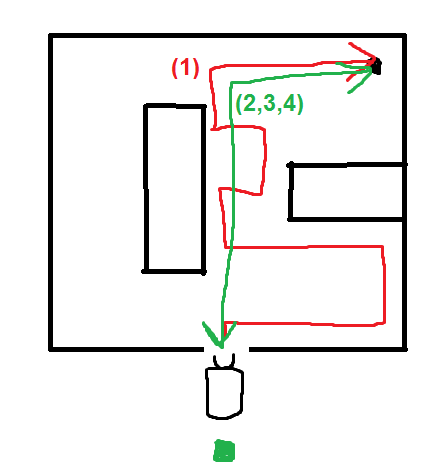
\includegraphics[scale=0.7]{anvandnings_exempel}\\
Figur 1. \textit{Exempel på en körning.}
\end{center}
\pagebreak
\subsection{Bakgrundsinformation}
Det kan finnas tillfällen då en robot behövs istället för en eller flera människor för att undsätta ett antal nödställda människor genom att skicka med mediciner eller förnödenheter i miljöer som är för farliga för människor att ta sig igenom. En prototyp för hur en sådan robot skulle kunna konstrueras ger en bra uppfattning om hur tillämpbara olika lösningar är.

\subsection{Definitioner}
Prioritetsnivåer på kraven anges med siffrorna 1, 2 respektive 3. Prioritetsnivåerna för respektive siffra innebär att kravet är: grundläggande, dvs dessa krav skall utföras, extrakrav, utförs om det finns tid kvar i budgeten efter att 1:orna har genomförts, och 3, utförs absolut sist, dock inte nödvändigt. Ett exempel följer:


\begin{center}
\begin{longtable}{|l|l|p{.70\linewidth}|l|} \hline
Krav nr A&
Original&
Ett krav som skall finnas med&
1 \\ \hline

Krav nr B&
Original &
Ett krav som utförs om tidsbudgeten tillåter &
2 \\ \hline

Krav nr C&
Original &
Ett krav som utförs om allt annat är gjort och projektgruppen känner för det.&
3 \\ \hline
\end{longtable}
\end{center}


\pagebreak

\section{Översikt av systemet}
Roboten består av ett chassi med bland annat tre moduler, nämligen en kommunikations-, styr-, samt sensormodul. Användaren och systemet kommunicerar via en dator. I chassit ingår dessutom motor, hjul och gripklo.

\begin{center}
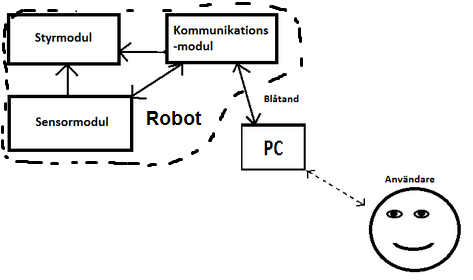
\includegraphics{systemskiss}

Figur 2. \textit{Denna bild visar en översikt av systemet.}
\end{center}

\subsection{Grov beskrivning av produkten}
Roboten kommer att köras på hjul och kommer att kunna känna av vad som finns framför, vid sidan av och bakom. Den ska kunna greppa tag i medicin eller annan produkt som roboten är avsedd att leverera. Den ska kunna kartlägga ett okänt område och utifrån kartan beräkna samt köra den kortaste vägen från start- till slutdestination. 

\subsection{Produktkomponenter}
Roboten kommer bestå av ett flertal olika sensorer med avståndsmätning. Minst tre stycken mikroprocessorer (en per delmodul). Roboten kommer att ha fyra hjul som alla drivs av motorer som går att kontrollera individuellt. Roboten kommer ha utrustning för att kunna greppa tag i en produkt.

\subsection{Beroenden till andra system}
Banan som roboten ska köra i måste uppfylla tävlingsreglerna (se bifogat dokument \textit{Banspecifikation och tävlingsregler})

\subsection{Ingående delsystem}
Roboten består av tre stycken delsystem (moduler). Kommunikationsmodul, styrmodul och sensormodul. Den förstnämnda sköter kommunikationen mellan roboten och en PC, denna kommunikation sköts via blåtand. Styrmodulen hanterar styrlogik och motorer. Sensormodulen skickar data till kommunikationsmodulen och styrmodulen som tar in dessa och korrigerar riktning efter datan.

\subsection{Avgränsningar}
Miljön som roboten körs i är begränsad på så sätt att den max ska vara 6x6m och passager måste vara bredare än 40 cm. Inga blockerande hinder får förekomma i vägen för roboten, den kan endast röra sig på släta ytor.

\subsection{Designfilosofi}
Målet är att roboten ska vara så snabb och energieffektiv som möjligt och samtidigt utföra uppgiften utan komplikationer. 

\subsection{Generella krav på hela systemet}
Nedan listas generella krav på hela systemet
\\
\begin{center}
\begin{longtable}{|l|l|p{.70\linewidth}|l|} \hline

Krav nr\kravcc & 
Original & 
Roboten ska kunna navigera autonomt i en labyrint. & 
1 \\ \hline

Krav nr\kravcc & 
Original & 
Roboten ska kunna röra sig framåt, framåt vänster, framåt höger, bakåt samt rotera vänster och höger. & 
1 \\ \hline

Krav nr\kravcc &
Original &
Sensorerna skall kunna kalibreras. &
1 \\ \hline

Krav nr\kravcc &
Original &
Kommandon ska ges via en PC via blåtand. &
1 \\ \hline

Krav nr\kravcc &
Original &
Roboten ska vara utrustad med en gripklo fram, vilken ska kunna plocka upp “förnödenheter” och lämna de på målrutan. &
1 \\ \hline

Krav nr\kravcc &
Original &
Roboten ska vara moduluppbyggd. &
1 \\ \hline

Krav nr\kravcc &
Original &
Modulerna skall vara utbytbara. &
1 \\ \hline

Krav nr\kravcc &
Original &
Varje modul ska innehålla minst en egen processor. &
1 \\ \hline

Krav nr\kravcc &
Original &
Det ska finnas en brytare på roboten för att växla mellan autonomt läge och fjärrstyrningsläge. &
1 \\ \hline

Krav nr\kravcc &
Original &
En knapp skall finnas som startar roboten i autonomt läge vid tävlingstillfället. &
1 \\ \hline

Krav nr\kravcc &
Original &
Styrmodul skall finnas. &
1 \\ \hline

Krav nr\kravcc &
Original &
Sensormodul skall finnas. &
1 \\ \hline

Krav nr\kravcc &
Original &
Kommunikationsmodul skall finnas. &
1 \\ \hline

Krav nr\kravcc &
Original &
Felmeddelanden ska vara på svenska &
1 \\ \hline

Krav nr\kravcc &
Original &
Roboten skall klara passager bredare större än 40 cm. &
2 \\ \hline
\end{longtable}
\end{center}

\pagebreak

\section{Delsystem 1 - Sensormodul}
Delsystem 1 är sensormodulen som består av minst en mikroprocessor samt de olika typer av sensorer som används för att mäta av robotens omgivning.


\subsection{Inledande beskrivning av delsystem 1}
Sensormodulen samlar in mätdata från sina olika sensorer och skickar denna data till styrmodulen (delsystem 2) där denna behandlas och eventuella åtgärder vidtas.

\begin{center}
\begin{longtable}{|l|l|p{.70\linewidth}|l|} \hline

Krav nr\kravcc & 
Original &
Information från sensormodulen ska skickas seriellt till andra moduler. Data ska vara angivet i SI-enheter &
1 \\ \hline

Krav nr\kravcc &
Original &
En LCD-skärm skall finnas på roboten och visa värden från sensorer kontinuerligt. &
2 \\ \hline

Krav nr\kravcc &
Original &
Roboten skall upptäcka mål som är utmärkt enligt en svart markering. &
1 \\ \hline

Krav nr\kravcc &
Original &
Roboten skall upptäcka mål som är utmärkt enligt en en RFID tag.&
2 \\ \hline

\end{longtable}
\end{center}


\section{Delsystem 2 - Styrmodul}
Styrmodulen ska bestå av minst en mikroprocessor.  Denna samlar information från sensor- och kommunikationsmodulerna, och agerar utefter svaren.


\subsection{Inledande beskrivning av delsystem 2}
Styrmodulen ska styra LCD:n, styrlogiken och motorerna.
LCD:n kommer att visa resultat som sensormodulen har skickat till styrmodulen. Styrlogiken kontrollerar motorerna och beroende på vad styrlogiken skickar för kommandon driver motorerna olika.

\begin{center}
\begin{longtable}{|l|l|p{.70\linewidth}|l|} \hline

Krav nr\kravcc &
Original &
Roboten ska kunna bestämma den kortaste vägen till målrutan. &
1 \\ \hline

Krav nr\kravcc &
Original &
Någon form av styralgoritm skall finnas. &
1 \\ \hline

Krav nr\kravcc &
Original &
Roboten skall klara passager bredare än 40 cm. &
2 \\ \hline

Krav nr\kravcc &
Original &
Roboten kan autonomt efter avsökning av labyrinten gripa tag i den enhet som ska levereras. &
2 \\ \hline

\end{longtable}
\end{center}


\pagebreak

\section{Delsystem 3 - Kommunikationsmodul}
Delsystem 3 är kommunikationsmodulen som sköter stor del av kommunikationen mellan de olika delsystemen. 
\begin{center}
\begin{longtable}{|l|l|p{.70\linewidth}|l|} \hline

Krav nr\kravcc &
Original &
Roboten ska kunna skicka mätdata (avstånd till väggar, avlagd sträcka, vridning), styrbeslut och styrdata till PC via blåtand. &
1 \\ \hline

\end{longtable}
\end{center}

\section{Delsystem 4 - PC}

PC:n används då data från roboten skall behandlas, och visas upp i ett användargränssnitt.
\\

\begin{center}
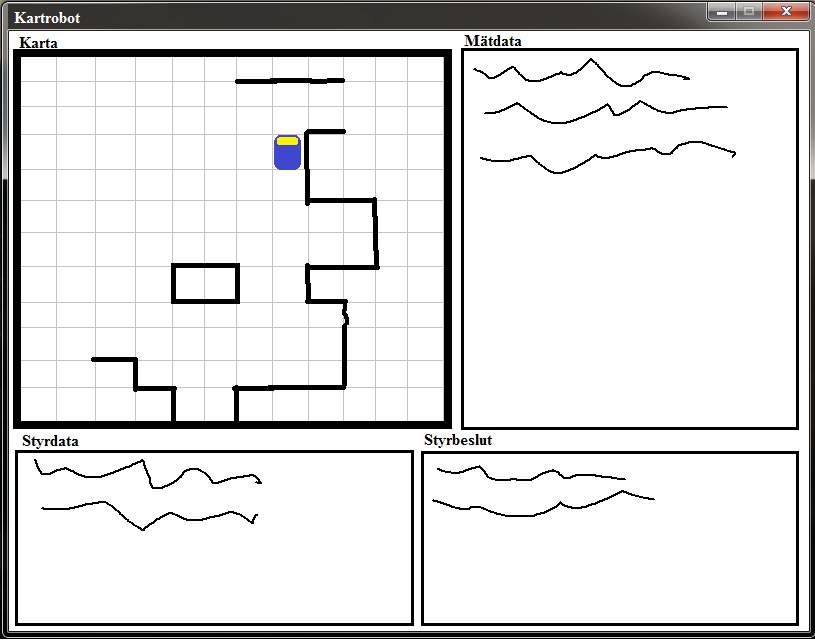
\includegraphics[scale=0.5]{anvandargranssnitt}

Figur 3. \textit{Skiss över användargränssnittet.}
\end{center}

\begin{center}
\begin{longtable}{|l|l|p{.70\linewidth}|l|} \hline

Krav nr\kravcc &
Original &
PC:n skall kunna ta emot data från kommunikationsmodulen via blåtand. &
1 \\ \hline

Krav nr\kravcc &
Original &
Data som visas på PC:n skall vara lätta att tolka och läsa av. &
1 \\ \hline

Krav nr\kravcc &
Original &
Kommandon ska ges till roboten från PC:n via blåtand. &
1 \\ \hline

Krav nr\kravcc &
Original &
Roboten bör kunna skicka positionsdata till PC. &
2 \\ \hline

Krav nr\kravcc &
Original &
En karta över grottan ska kunna presenteras på en monitor/projektor utifrån den data som har samlats in. &
2 \\ \hline
\end{longtable}
\end{center}


\section{Prestandakrav}
Prestandakrav ställs för att garantera en robot som klarar av att utföra uppdraget med tillfredsställande resultat samt även för att garantera en viss grad av användandenytta.

\begin{center}
\begin{longtable}{|l|l|p{.70\linewidth}|l|} \hline

Krav nr\kravcc &
Original &
Roboten skall klara av upprepade (upp till 3) uppdrag utan driftproblem (laddning av batteri räknas ej till detta). &
2 \\ \hline

\end{longtable}
\end{center}

\section{Krav på vidareutveckling}
Utöver krav nr 6 så ställs inga krav på vidareutveckling.

\section{Tillförlitlighet}
För att öka robotens användandenytta ställs krav på tillförlitligheten hos roboten.

\begin{center}
\begin{longtable}{|l|l|p{.70\linewidth}|l|} \hline

Krav nr\kravcc &
Original &
Roboten skall klara av att utforska olika labyrinter. &
1 \\ \hline

\end{longtable}
\end{center}

\section{Ekonomi}
De resurser som finns att tillgå är 1360 timmar fördelat på gruppens 6 medlemmar. 

\begin{center}
\begin{longtable}{|l|l|p{.70\linewidth}|l|} \hline

Krav nr\kravcc &
Original &
Projektet får ta maximalt 1380 arbetstimmar att utföra efter godkänd plan. &
1 \\ \hline
\end{longtable}
\end{center}

\section{Krav på säkerhet}
Roboten ska uppfylla följande krav när det gäller säkerhet:

\begin{center}
\begin{longtable}{|l|l|p{.70\linewidth}|l|} \hline

Krav nr\kravcc &
Original &
Roboten skall inte kollidera med några hinder i labyrinten. &
1 \\ \hline

\end{longtable}
\end{center}

\pagebreak
\section{Leveranskrav och delleveranser}
Leveranser skall göras senast på nedan nämnda tider och datum om inte annat är överenskommet mellan beställare och projektgrupp
\begin{center}
\begin{longtable}{|l |p{.8\linewidth}|} \hline

3 feb: & 
kl 16.00: Kravspecifikationen ska vara klar. (BP1) \\ \hline

16 feb: & 
kl 16.00: Första versionen av projektplan, tidplan och systemskiss ska vara inlämnade till beställaren. \\ \hline

20 feb: & 
kl 16.00: Slutgiltig version av projektplan, tidplan och systemskiss ska vara inlämnade till beställaren. \\ \hline

5 mars: &
kl 16.00: första version av förstudien (minst 5 sidor) ska skickas till respektive handledare och till er beställare. \\ \hline

11 mars: & 
kl 16.00: Första versionen av designspecifikationen ska vara inlämnad till handledaren. \\ \hline

24 mars: &
Designspecifikationen ska vara godkänd av handledaren vid ett beslutsmöte BP3. \\ \hline

1 april: &
kl 16:00 Version 1.0 av förstudien ska skickas till respektive handledare och till beställare. \\ \hline

17 april: & 
Nuvarande design ska vara presenterad för och godkänd av handledaren vid ett beslutsmöte BP4. \\ \hline

25 maj: &
Verifiering av kraven (BP5) bör ske i god tid innan redovisningen. Utan detta beslut får ni inte leverera! \\ \hline

21 maj: &
Kappan, version 1.0, (exklusive appendix) ska levereras. Se nedan. \\ \hline

27 maj: &
Teknisk dokumentation och användarhandledning (båda version 1.0) ska vara inlämnade. Slutversion av skrivarbete skall också skickas med vid detta tillfälle. \\ \hline

Vecka 23: &
Redovisning och demonstration.\\ \hline

2 juni: &
(preliminärt) 8.15-17 muntliga presentationer och opposition. Tider se nedan. \\ \hline

3 juni: &
(preliminärt) 9.15-17 tävlingar utanför café Java. \\ \hline

5 juni: &
Efterstudien ska vara inlämnad. Vid denna tidpunkt ska även källkod skickas in i en zip-fil. \\ \hline

12 juni: &
Bärbar dator och övrig utrustning ska vara återlämnade. \\ \hline
\end{longtable}
\end{center}
En tidrapport ska lämnas senast kl 16.00 vid följande datum: 4 febr, 23 febr, 9 mars, 23 mars, 30 mars, 13 april, 20 april, 27 april, 4 maj, 11 maj, 18 maj, 25 maj, 1 juni och 8 juni.

\begin{center}
\begin{longtable}{|l|l|p{.70\linewidth}|l|} \hline

Krav nr\kravcc &
Original &
Vid slutleverans, 27/5, skall en fungerande robot finnas. &
1 \\ \hline

\end{longtable}
\end{center}


\pagebreak

\section{Dokumentation}
Följande tabell räknar upp de dokument som kommer att skapas under projektets gång, samt deras syfte.
\begin{center}
\begin{longtable}{|p{.24\linewidth}|p{.08\linewidth}|p{.25\linewidth}|p{.19\linewidth}|p{.1\linewidth}|}\hline
\textbf{Dokument} & \textbf{Språk} & \textbf{Syfte} & \textbf{Målgrupp} & \textbf{Format} \\ \hline

Kravspecifikation & SE & Listar alla krav som slutprodukten ska uppfylla. & Projektgrupp och beställare & .pdf \\ \hline
Projektplan & SE & Beskriver hur projektet ska utföras & Projektgrupp & .pdf \\ \hline
Tidplan & SE & Beskriver när aktiviteter ska utföras och av vem & Projektgrupp & .xls \\ \hline
Systemskiss & SE & Beskriver hur produkten ska konstrueras& Projektgrupp och beställare & .pdf \\ \hline
Förstudie & SE & Analysera huruvida projektet kan drivas framåt eller inte & Projektgrupp & .pdf \\ \hline
Design-specifikation & SE & Beskriver mer detaljerat hur produkten ska konstrueras & Projektgrupp & .pdf \\ \hline
Kappa & SE & Sammanfattar alla dokument som beställaren kan vara intresserad av & Beställare & .pdf \\ \hline
Teknisk dokumentation & SE & Beskriver hur produkten fungerar & Beställare & .pdf \\ \hline
Användar-handledning & SE & Beskriver hur man använder produkten& Beställare & .pdf \\ \hline
Efterstudie & SE & En reflektion kring hur projektet bedrevs. Vad kunde man ha gjort bättre, etc.& Projektgrupp & .pdf \\ \hline

\end{longtable}
\end{center}

\section{Utbildning}
Vid slutfört projekt skall en utförlig teknisk dokumentation av hela systemet samt alla ingående delsystem finnas. Det skall också finnas en godkänd användarhandledning att tillgå vid projektets slutleverans som ska garantera kunden tillräcklig kunskap för användande av roboten.

\section{Kvalitetskrav}
Kvalitetskrav ställer krav på robotens pålitlighet samt stabilitet hos program och komponenter i systemet.

\section{Underhållsbarhet}
För att garantera robotens funktionalitet för en översiktlig framtid ska underlag för underhåll finnas i någon form.

\setcounter{secnumdepth}{0}
\pagebreak
\section{Referenser}
Banspecifikation och tävlingsregler \\
Banspecifikation och tävlingsregler v0.1.pdf
\\[0.1in]
Projektdirektiv för en undsättningsrobot, Tomas Svensson
http://www.isy.liu.se/edu/kurs/TSEA56/Dokument/Projektdirektiv\%20undsattningsrobot\_15.pdf

\setcounter{secnumdepth}{2}



\end{flushleft}




\end{document}

